\documentclass{beamer}

\mode<presentation> {

%\usetheme{default}
%\usetheme{AnnArbor}
%\usetheme{Antibes}
%\usetheme{Bergen}
%\usetheme{Berkeley}
%\usetheme{Berlin}
%\usetheme{Boadilla}
%\usetheme{CambridgeUS}
%\usetheme{Copenhagen}
%\usetheme{Darmstadt}
%\usetheme{Dresden}
%\usetheme{Frankfurt}
%\usetheme{Goettingen}
%\usetheme{Hannover}
%\usetheme{Ilmenau}
%\usetheme{JuanLesPins}
%\usetheme{Luebeck}
\usetheme{Madrid}
%\usetheme{Malmoe}
%\usetheme{Marburg}
%\usetheme{Montpellier}
%\usetheme{PaloAlto}
%\usetheme{Pittsburgh}
%\usetheme{Rochester}
%\usetheme{Singapore}
%\usetheme{Szeged}
%\usetheme{Warsaw}


%\usecolortheme{albatross}
%\usecolortheme{beaver}
%\usecolortheme{beetle}
%\usecolortheme{crane}
%\usecolortheme{dolphin}
%\usecolortheme{dove}
%\usecolortheme{fly}
%\usecolortheme{lily}
%\usecolortheme{orchid}
%\usecolortheme{rose}
%\usecolortheme{seagull}
%\usecolortheme{seahorse}
%\usecolortheme{whale}
%\usecolortheme{wolverine}

%\setbeamertemplate{footline} % To remove the footer line in all slides uncomment this line
%\setbeamertemplate{footline}[page number] % To replace the footer line in all slides with a simple slide count uncomment this line

%\setbeamertemplate{navigation symbols}{} % To remove the navigation symbols from the bottom of all slides uncomment this line
}

\usepackage{graphicx} % Allows including images
\usepackage{booktabs} % Allows the use of \toprule, \midrule and \bottomrule in tables
\usepackage{amsfonts}
\usepackage{mathrsfs, bbold}
\usepackage{amsmath,amssymb,graphicx}
\usepackage{mathtools} % gather
\usepackage[export]{adjustbox} % right-aligned graphics

% argmax
\DeclareMathOperator*{\argmax}{arg\,max}

%----------------------------------------------------------------------------------------
%	TITLE PAGE
%----------------------------------------------------------------------------------------

\title["22"]{22: Finite Mixture Models}

\author{Taylor} 
\institute[UVA] 
{
University of Virginia \\
\medskip
\textit{} 
}
\date{} 

\begin{document}
%----------------------------------------------------------------------------------------

\begin{frame}
\titlepage 
\end{frame}

%----------------------------------------------------------------------------------------
\begin{frame}
\frametitle{Introduction}

We'll take a look at {\bf finite mixture models} now, and see how they're useful for mixture modeling.

\end{frame}

%----------------------------------------------------------------------------------------
\begin{frame}
\frametitle{Introduction}

\begin{center}
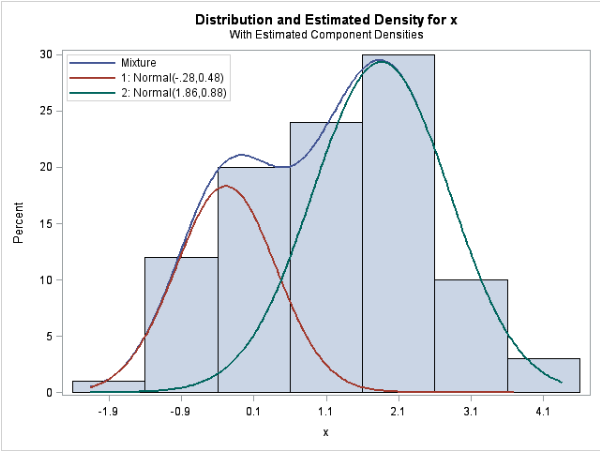
\includegraphics[width=45mm]{mixpic1.png}
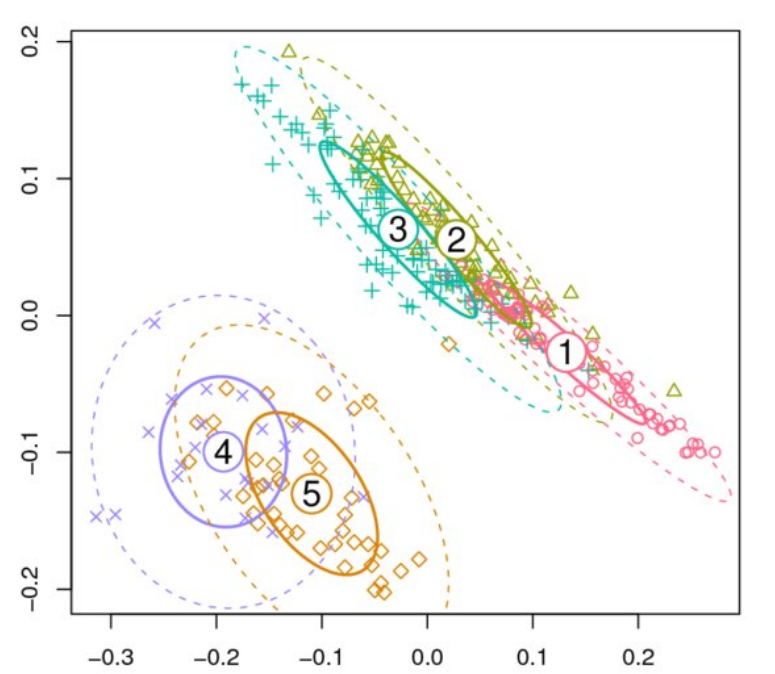
\includegraphics[width=45mm]{mixpic2.png}
\end{center}

\end{frame}

%----------------------------------------------------------------------------------------
\begin{frame}
\frametitle{Notation}


\begin{enumerate}
\item $H$ is the number of mixtures ($h=1, \ldots, H$)
\item $\theta = (\theta_1, \ldots, \theta_H)$ parameters for each mixture
\item $z_i = (z_{i1}, \ldots, z_{ih})$ missing data aka indicator/one-hot vector 
\item $\lambda = (\lambda_1, \ldots, \lambda_H)$ parameter for $p(z_i \mid \lambda)$
\end{enumerate}
and
\begin{enumerate}
\item $p(z_i \mid \lambda)$ distribution over missing data 
\item $f(y_i \mid \theta_h)$ mixture-specific densities
\item $p(y_i \mid z_i, \theta) = \prod_{h=1}^Hf(y_i \mid \theta_h)^{z_{ih}} $
\end{enumerate}

\end{frame}

%----------------------------------------------------------------------------------------
\begin{frame}
\frametitle{Notation}

Typically
\begin{align*}
p(z_i \mid \lambda) &= \prod_{h=1}^H \lambda_h^{z_{ih}} 
\end{align*}
(for example $z_i =  [z_{i1},  \ldots, z_{ih}]= [0, \ldots, 1, \ldots, 0]$) and
\begin{align*}
p(y_i \mid z_i, \theta) &= \sum_{i=1}^H 1_{z_{ih}=1} f(y_i \mid \theta_h) \\
&= \prod_{h=1}^H f(y_i \mid \theta_h)^{z_{ih} }
\end{align*}
so
$$
p(y_i , z_i \mid \theta, \lambda) = p(y_i \mid z_i, \theta) p(z_i \mid \lambda) = \prod_{h=1}^H \lambda_h^{z_{ih}} f(y_i \mid \theta_h)^{z_{ih} }
$$

\end{frame}
%----------------------------------------------------------------------------------------
\begin{frame}
\frametitle{Identifiability and Label-switching}

The observed data likelihood isn't identifiable because
\begin{align*}
p(y_i \mid \theta, \lambda) &= \sum_{z_i} p(y_i \mid z_i, \theta) p(z_i \mid \lambda) \\
&= \sum_{z_i} \prod_{h=1}^H \lambda_h^{z_{ih}} f(y_i \mid \theta_h)^{z_{ih} } \\
&= \sum_{h} \lambda_h f(y_i \mid \theta_h) \\
&= \sum_{h} \lambda_h' f(y_i \mid \theta_h') \\
&= p(y_i \mid \theta', \lambda')
\end{align*}


where $\theta'$ and $\lambda'$ are just permuted versions of $\theta$ and $\lambda$ respectively.

\end{frame}

%----------------------------------------------------------------------------------------
\begin{frame}
\frametitle{Identifiability and Label-switching}

Watch out for exchangeable priors!
\newline

If the prior is exchangeable and the likelihood is not identifiable, then the posterior will be exchangeable:
\begin{align*}
p(\theta, \lambda) p(y \mid \theta, \lambda) &= p(\theta, \lambda) p(y \mid \theta', \lambda') \tag{label switching} \\
&= p(\theta', \lambda') p(y \mid \theta', \lambda') \tag{exchangeable prior}
\end{align*}
\pause

This means that there is no information about mixture-specific parameters.
\end{frame}
%----------------------------------------------------------------------------------------
\begin{frame}
\frametitle{Gibbs sampling}

In a Gibbs sampling algorithm, we alternate between sampling from these conditionals:
\begin{enumerate}
\item $p(z \mid y, \theta, \lambda) $
\item $p(\theta, \lambda \mid z, y)$
\end{enumerate}
where $y = (y_1, \ldots, y_n)$ and $z = (z_1, \ldots, z_n)$ (an $n \times h$ matrix)


\end{frame}


%----------------------------------------------------------------------------------------
\begin{frame}
\frametitle{Gibbs sampling}

\begin{align*}
p(z \mid y, \theta, \lambda) &\propto p(\theta, \lambda)\prod_{i=1}^n p(y_i \mid z_i, \theta) p(z_i \mid \lambda) \\
&\propto \prod_{i=1}^n p(y_i \mid z_i, \theta) p(z_i \mid \lambda) \\
&= \prod_{i=1}^n \prod_{h=1}^H \left[ \lambda_h f(y_i \mid \theta_h)\right]^{z_{ih} } \\
\end{align*}

So each $z_i$ is Multinomial with probabilities proportional to
$$
[\lambda_1 f(y_i \mid \theta_1)], \ldots, [\lambda_H f(y_i \mid \theta_H)]
$$
\end{frame}

%----------------------------------------------------------------------------------------
\begin{frame}
\frametitle{Gibbs sampling}

For the other conditional posterior:
\begin{align*}
p(\theta, \lambda \mid z, y) &\propto p(\theta, \lambda )p(y \mid z, \theta)p(z \mid \lambda) \\
\end{align*}

Note if $p(\theta, \lambda) = p(\theta)p(\lambda)$, then the posterior factors, too. 
\newline

You can't really say any more without more details on the model. 

\end{frame}

%----------------------------------------------------------------------------------------
\begin{frame}
\frametitle{Gibbs sampling: Example}

Instead of a one-hot representation, we'll use $z_i \in \{1,\ldots,H\}$.
\newline
\pause



Here's the complete-data likelihood:

\begin{enumerate}
\item $f(y_i \mid \theta_h) = \frac{1}{\sqrt{2\pi \tau^2_{h} }}\exp\left[-\frac{(y_i - \mu_{h} )^2 }{ 2\tau^2_{h} } \right]$
\item $p(y_i \mid z_i, \theta) = \prod_{h} [f(y_i \mid \theta_h)]^{z_{ih}}$
\item $p(z_i = h \mid \lambda) = \lambda_h$
\item $p(z_i \mid \lambda) = \prod_h \lambda_h^{z_{ih}}$
\end{enumerate}
\pause

The priors for $(\theta_1, \ldots, \theta_H) = (\mu_1, \tau^2_1, \ldots, \mu_H, \tau^2_H)$ require us to pick $\mu_0$, $\kappa$, $a_{\tau}$, and $b_{\tau}$:
\begin{enumerate}
\item $p(\mu_h \mid \tau^2_{h}) = \frac{1}{\sqrt{2\pi \kappa \tau^2  }}\exp\left[-\frac{(\mu_{h} -  \mu_0)^2 }{ 2\kappa \tau_h^2 } \right]$
\item $p(\tau^2_{h}) = \text{Inv-Gamma}(a_{\tau}, b_{\tau})$.
\end{enumerate}
\pause

Last, 
\begin{enumerate}
\item $p(\lambda_1, \ldots, \lambda_H) \propto \prod_{h=1}^H \lambda^{a_h-1}$
\end{enumerate}

\end{frame}

%----------------------------------------------------------------------------------------
\begin{frame}
\frametitle{Gibbs sampling: Example}

Overview: we derive the following two distributions
\begin{enumerate}
\item $p(z \mid y, \theta, \lambda) $
\item $p(\theta, \lambda \mid z, y) = p(\theta \mid z, y)p(\lambda \mid z, y)$.
\end{enumerate}
The second distribution factors by the reasoning we used in slide 10.


\end{frame}
%----------------------------------------------------------------------------------------
\begin{frame}[fragile]
\frametitle{Gibbs sampling: Example}

Continuing on now with specific distributions...
\begin{align*}
p(z \mid y, \theta, \lambda) &\propto \prod_{i=1}^n \prod_{h=1}^H \left[ \lambda_h f(y_i \mid \theta_h)\right]^{z_{ih} } \\
&= \prod_{i=1}^n \prod_{h=1}^H \left[ \lambda_h \frac{1}{\sqrt{2\pi \tau^2_{h} }}\exp\left[-\frac{(y_i - \mu_{h} )^2 }{ 2\tau^2_{h} } \right] \right]^{z_{ih} }
\end{align*}

Programming this will be easier, though, if you use \verb|dnorm| and \verb|rmultinom|.

\end{frame}
%----------------------------------------------------------------------------------------
\begin{frame}[fragile]
\frametitle{Gibbs sampling: Example}

Continuing on now with specific distributions...
\newline

\begin{align*}
p(\lambda \mid z, y) &\propto p(\theta)p(\lambda )p(y \mid z, \theta)p(z \mid \lambda) \\
&\propto p(\lambda )p(z \mid \lambda) \\
&\propto \left[\prod_{h=1}^H   \lambda^{a_h-1}\right] \left[\prod_{i=1}^n  \prod_{h=1}^H \lambda_h^{z_{ih}} \right] \\
&= \prod_{h=1}^H \lambda^{a_h + n_h -1}
\end{align*}
where $n_h = \sum_{i=1}^n 1_{z_{i} = h }$


\end{frame}

%----------------------------------------------------------------------------------------
\begin{frame}[fragile]
\frametitle{Gibbs sampling: Example}

Continuing on now with specific distributions...
\begin{align*}
p(\theta \mid z, y) &\propto p(\theta)p(\lambda )p(y \mid z, \theta)p(z \mid \lambda) \\
&\propto p(\theta)p(y \mid z, \theta) \\
&\propto p(\mu, \tau^2)p(y \mid z, \mu, \tau^2) 
\end{align*}
where $\mu = (\mu_1, \ldots, \mu_H)$, $\tau^2 = (\tau^2_1, \ldots, \tau^2_H)$, and $n_h = \sum_{i=1}^n 1_{z_{i} = h }$.

% &\propto \left[\prod_{h=1}^H p(\mu_h \mid \tau^2_{h})p(\tau^2_{h})  \right] \left[\prod_{i=1}^n  \prod_{h=1}^H  f(y_i \mid \theta_h)^{z_{ih}} \right] \\
% &\propto \left[\prod_{h=1}^H p(\mu_h \mid \tau^2_{h})p(\tau^2_{h})  \right] \left[\prod_{i=1}^n  \prod_{h=1}^H  f(y_i \mid \mu_h, \tau^2_h)^{z_{ih}} \right] 




\end{frame}


%----------------------------------------------------------------------------------------
\begin{frame}[fragile]
\frametitle{Gibbs sampling: Example}

The ``Normal" part of the Normal-Inverse-Gamma:
\begin{align*}
p(\mu, \tau^2 \mid z, y) &\propto p(\mu, \tau^2)p(y \mid z, \mu, \tau^2) \\
&= \left[\prod_{h=1}^H p(\mu_h \mid \tau^2_{h})p(\tau^2_{h})  \right] \left[\prod_{i=1}^n  \prod_{h=1}^H  f(y_i \mid \mu_h, \tau^2_h)^{z_{ih}} \right].
\end{align*}
\pause

For each $h$
\begin{align*}
p(\mu_h, \tau^2_h)p(y \mid z, \mu_h, \tau_h^2) &=  p(\mu_h \mid \tau^2_{h})p(\tau^2_{h})  \prod_{i=1}^n   f(y_i \mid \mu_h, \tau^2_h)^{z_{ih}}.
\end{align*}

will be a Normal-Inverse-Gamma distribution. 


\end{frame}


%----------------------------------------------------------------------------------------
\begin{frame}[fragile]
\frametitle{Gibbs sampling: Example}

The ``Normal" part of the Normal-Inverse-Gamma (continued)

\begin{align*}
&p(\mu_h \mid \tau^2_h, y, z) \\
&\propto p(\mu_h \mid \tau^2_{h})  \prod_{i=1}^n   f(y_i \mid \mu_h, \tau^2_h)^{z_{ih}}\\
&\propto \frac{1}{\sqrt{2\pi \kappa \tau^2  }}\exp\left[-\frac{(\mu_{h} -  \mu_0)^2 }{ 2\kappa \tau_h^2 } \right] \prod_{i=1}^n \left[ \frac{1}{\sqrt{2\pi \tau^2_{h} }}\exp\left[-\frac{(y_i - \mu_{h} )^2 }{ 2\tau^2_{h} } \right] \right]^{z_{ih}} \\
&\propto \exp\left[-\frac{1}{2}\left\{  \frac{(\mu_{h} -  \mu_0)^2 }{ \kappa \tau_h^2 }  + \frac{\sum_{i : z_i = h}(y_i - \mu_{h} )^2 }{ \tau^2_{h} } \right\}\right]
\end{align*}

For more info see page 534.

% Also, we'll look at
% \begin{align*}
% &p(\mu_h \mid \tau^2_{h})p(\tau^2_{h})  \prod_{i=1}^n  f(y_i \mid \mu_h, \tau^2_h)^{z_{ih}} \right] \\
% &\propto  \frac{1}{\sqrt{2\pi \kappa \tau^2  }}\exp\left[-\frac{(\mu_{h} -  \mu_0)^2 }{ 2\kappa \tau_h^2 } \right] \left[(\tau^2)^{-(a_{\tau}+1)}\exp\left[ -\frac{b_{\tau} }{\tau^2} \right] \right]   \times \\
% &\hspace{10mm} \left[ \frac{1}{\sqrt{2\pi \tau^2_{h} }}\exp\left[-\frac{(y_i - \mu_{h} )^2 }{ 2\tau^2_{h} } \right] \right]^{n_h}
% \end{align*}

% p(\mu, \tau^2)p(y \mid z, \mu, \tau^2) 
\end{frame}


%----------------------------------------------------------------------------------------
\begin{frame}[fragile]
\frametitle{Gibbs sampling: Example}

The ``Inverse-Gamma" part of the Normal-Inverse-Gamma 

\begin{align*}
&p(\tau^2_h \mid  y, z) \\
&\propto p(\mu_h \mid \tau^2_{h})p(\tau^2_{h})  \prod_{i=1}^n   f(y_i \mid \mu_h, \tau^2_h)^{z_{ih}}\\
&\propto \frac{1}{\sqrt{2\pi \kappa \tau^2  }}\exp\left[-\frac{(\mu_{h} -  \mu_0)^2 }{ 2\kappa \tau_h^2 } \right] (\tau^2)^{-(a_{\tau}+1) } \exp\left[ - \frac{b_{\tau}}{\tau_h^2} \right] \times\\
&\hspace{10mm}\prod_{i=1}^n \left[ \frac{1}{\sqrt{2\pi \tau^2_{h} }}\exp\left[-\frac{(y_i - \mu_{h} )^2 }{ 2\tau^2_{h} } \right] \right]^{z_{ih}} \\
&\propto \exp\left[-\left\{ b_\tau +  \frac{(\mu_{h} -  \mu_0)^2 }{ 2\kappa  }  + \frac{\sum_{i : z_i = h}(y_i - \mu_{h} )^2 }{ 2 } \right\} \frac{1}{\tau^2_h} \right] (\tau^2)^{-\left( \frac{n_h}{2} + \alpha_{\tau} + 1 \right)-1/2 }
\end{align*}

\end{frame}


\end{document} 
